\section{Retrieval Coordination and Analysis Method}
Figure~\ref{fig:methodology} links the mission specification, URDF chain and actuator gateways to three offline studies: coordinator verification, wrist geometry and command semantics. Their evidence identifies integration requirements for subsequent physical trials.

\HazBotMethodologyFigure
\subsection{Mission and Evidence Contracts}
The reference mission has seven phases (Fig.~\ref{fig:mission}): SEARCH authorizes a candidate; APPROACH reaches its pickup region; DOCK transfers control from base to arm; GRASP secures the object; CARRY transports it with the arm stowed; PLACE releases it at the deposit region; and COMPLETE requires a release indication.


\begin{figure*}[t]
\centering
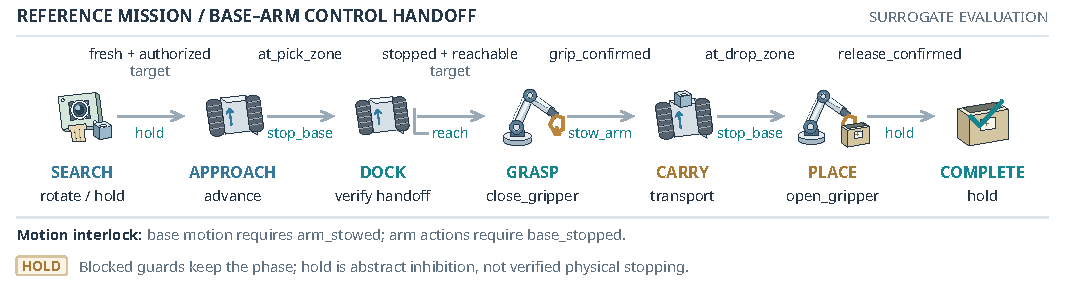
\includegraphics[width=\textwidth]{hazbot_mission.pdf}
\caption{Seven-phase reference retrieval mission. Conditions summarize the handoff evidence; complete command predicates are defined in the text and executable model. A failed prerequisite requests HOLD at the current phase. The strip depicts the coordination specification, rather than a measured physical trajectory.}
\label{fig:mission}
\end{figure*}

Let $T$ denote an authorized, fresh target; $S$ a fresh, usable scan; $C$ a clear route; $A$ a stowed arm and $B$ a stopped base. The principal command contracts are
\begin{align}
\text{base motion} &\Rightarrow S\land C\land A,\label{eq:baseguard}\\
\text{target approach} &\Rightarrow T,\\
\text{arm motion} &\Rightarrow B.\label{eq:armguard}
\end{align}
Reach and closure additionally require $T$ and wrist reachability; release requires the deposit region and a grip indication. The controller also requires scan health during docking, grasping and placement. A failed prerequisite emits HOLD without advancement. HOLD inhibits active motion and needs an explicit actuator-boundary stop. Target acquisition and release may advance phase while emitting HOLD. A stop request does not establish $B$: deployment requires measured base-rest feedback and a defined confirmation rule.

The abstract observations comprise twelve Boolean values: target authorization and freshness; scan freshness and usability; route clearance; arm stowage; base stopped; wrist reachability; pickup-region arrival; grip confirmation; deposit-region arrival and release confirmation. Each has a specific role in the interface but this discrete model does not generate these observations from physical sensors. In particular, grip and release indications are input assumptions, not inferred force or contact measurements.

\subsection{Bounded Reference-Model Verification}
The verification procedure in Fig.~\ref{fig:verification} enumerates every observation valuation at every phase: $7\times2^{12}=28{,}672$ phase--observation pairs per policy. No valuations are pruned. A separate admissibility oracle checks the output action against Eqs.~\ref{eq:baseguard}--\ref{eq:armguard} and the target, reach and placement conditions. Breadth-first exploration establishes phase reachability and extracts shortest-prefix counterexamples. Three ablations remove the base--arm interlock, target authorization or scan-age requirement from the controller while retaining the full oracle. This design tests whether each omitted condition creates a concrete contract violation.

All Boolean valuations are retained, including physically inconsistent combinations. Counts therefore describe the specification domain, not robot failure probabilities. A nominal trace checks progression to COMPLETE under admissible observations; neither it nor existential phase reachability establishes physical mission success.

\HazBotVerificationFigure

\subsection{Source-Derived Wrist Geometry}
Figure~\ref{fig:workspace} connects arm geometry to the docking prerequisite. From the URDF chain, the shoulder lies at $(0.100,0,0.155)$\,m in the base frame and both positioning links have length $L_1=L_2=0.100$\,m. The zero pose has a vertical upper link and horizontal forearm. The figure uses $q_1=q_b$, $q_2=q_s$, and $q_3=q_e$. For yaw $q_b$, shoulder angle $q_s$, and elbow angle $q_e$, the wrist origin is
\begin{align}
r &=L_1\sin q_s+L_2\cos(q_s+q_e),\\
x &=0.100+r\cos q_b,\quad y=r\sin q_b,\\
z &=0.155+L_1\cos q_s-L_2\sin(q_s+q_e).
\label{eq:fk}
\end{align}
We sample 41 values, including both bounds, for each positioning joint. The declared bounds are $q_b\in[-1.5708,1.5708]$, $q_s\in[-0.5,2.6179]$, and $q_e\in[-1.5708,2.6179]$\,rad. An independent homogeneous-transform implementation evaluates the URDF chain at 1,000 seeded random poses and 13 special poses. Agreement checks numerical implementation, while the grid characterizes the ideal wrist envelope. The wrist origin is not a calibrated grasp contact point; collision, load, compliance and stability constraints are not represented.

\begin{figure}[t]
\centering
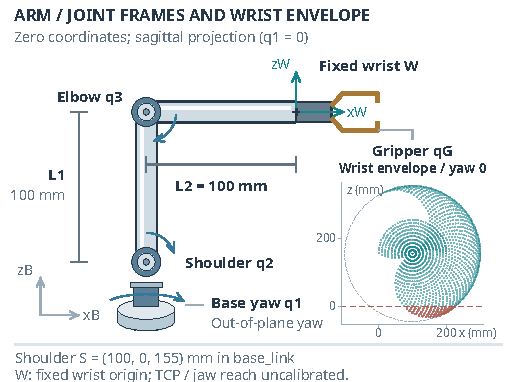
\includegraphics[width=\columnwidth]{hazbot_arm_geometry.pdf}
\caption{Source-derived arm geometry at zero joint coordinates, with joint axes and fixed wrist origin. The small inset shows 1,681 zero-yaw wrist samples, the link-sum bound, and modeled ground exclusions. Samples describe ideal geometry rather than calibrated contact positions or collision-free grasps.}
\label{fig:workspace}
\end{figure}

\subsection{Command-Interface Characterization}
Using Python's abstract syntax tree, we isolate the \code{SET:} branch of the actual wheel gateway and replace only the transport sender with an in-memory recorder. All integer pairs $(l,r)\in[-255,255]^2$ are executed and compared with an independently specified sign partition. The arm gateway's pure angle mapper is evaluated for five accepted aliases over 451 inputs from $-90$ to $360$, checking clamps and reversals. The elbow has two aliases, so this represents four actuator channels. No ROS constructors, sockets, motor servers or hardware launchers are executed. Source hashes, settings, CSV outputs and validation records bind the results to the analyzed implementation.
